\section{ 处理GPIO的相关函数 }
\subsection{ GPIO初始化函数,用于配置GPIO模式和引脚 }
\begin{figure}[h]
    \centering
    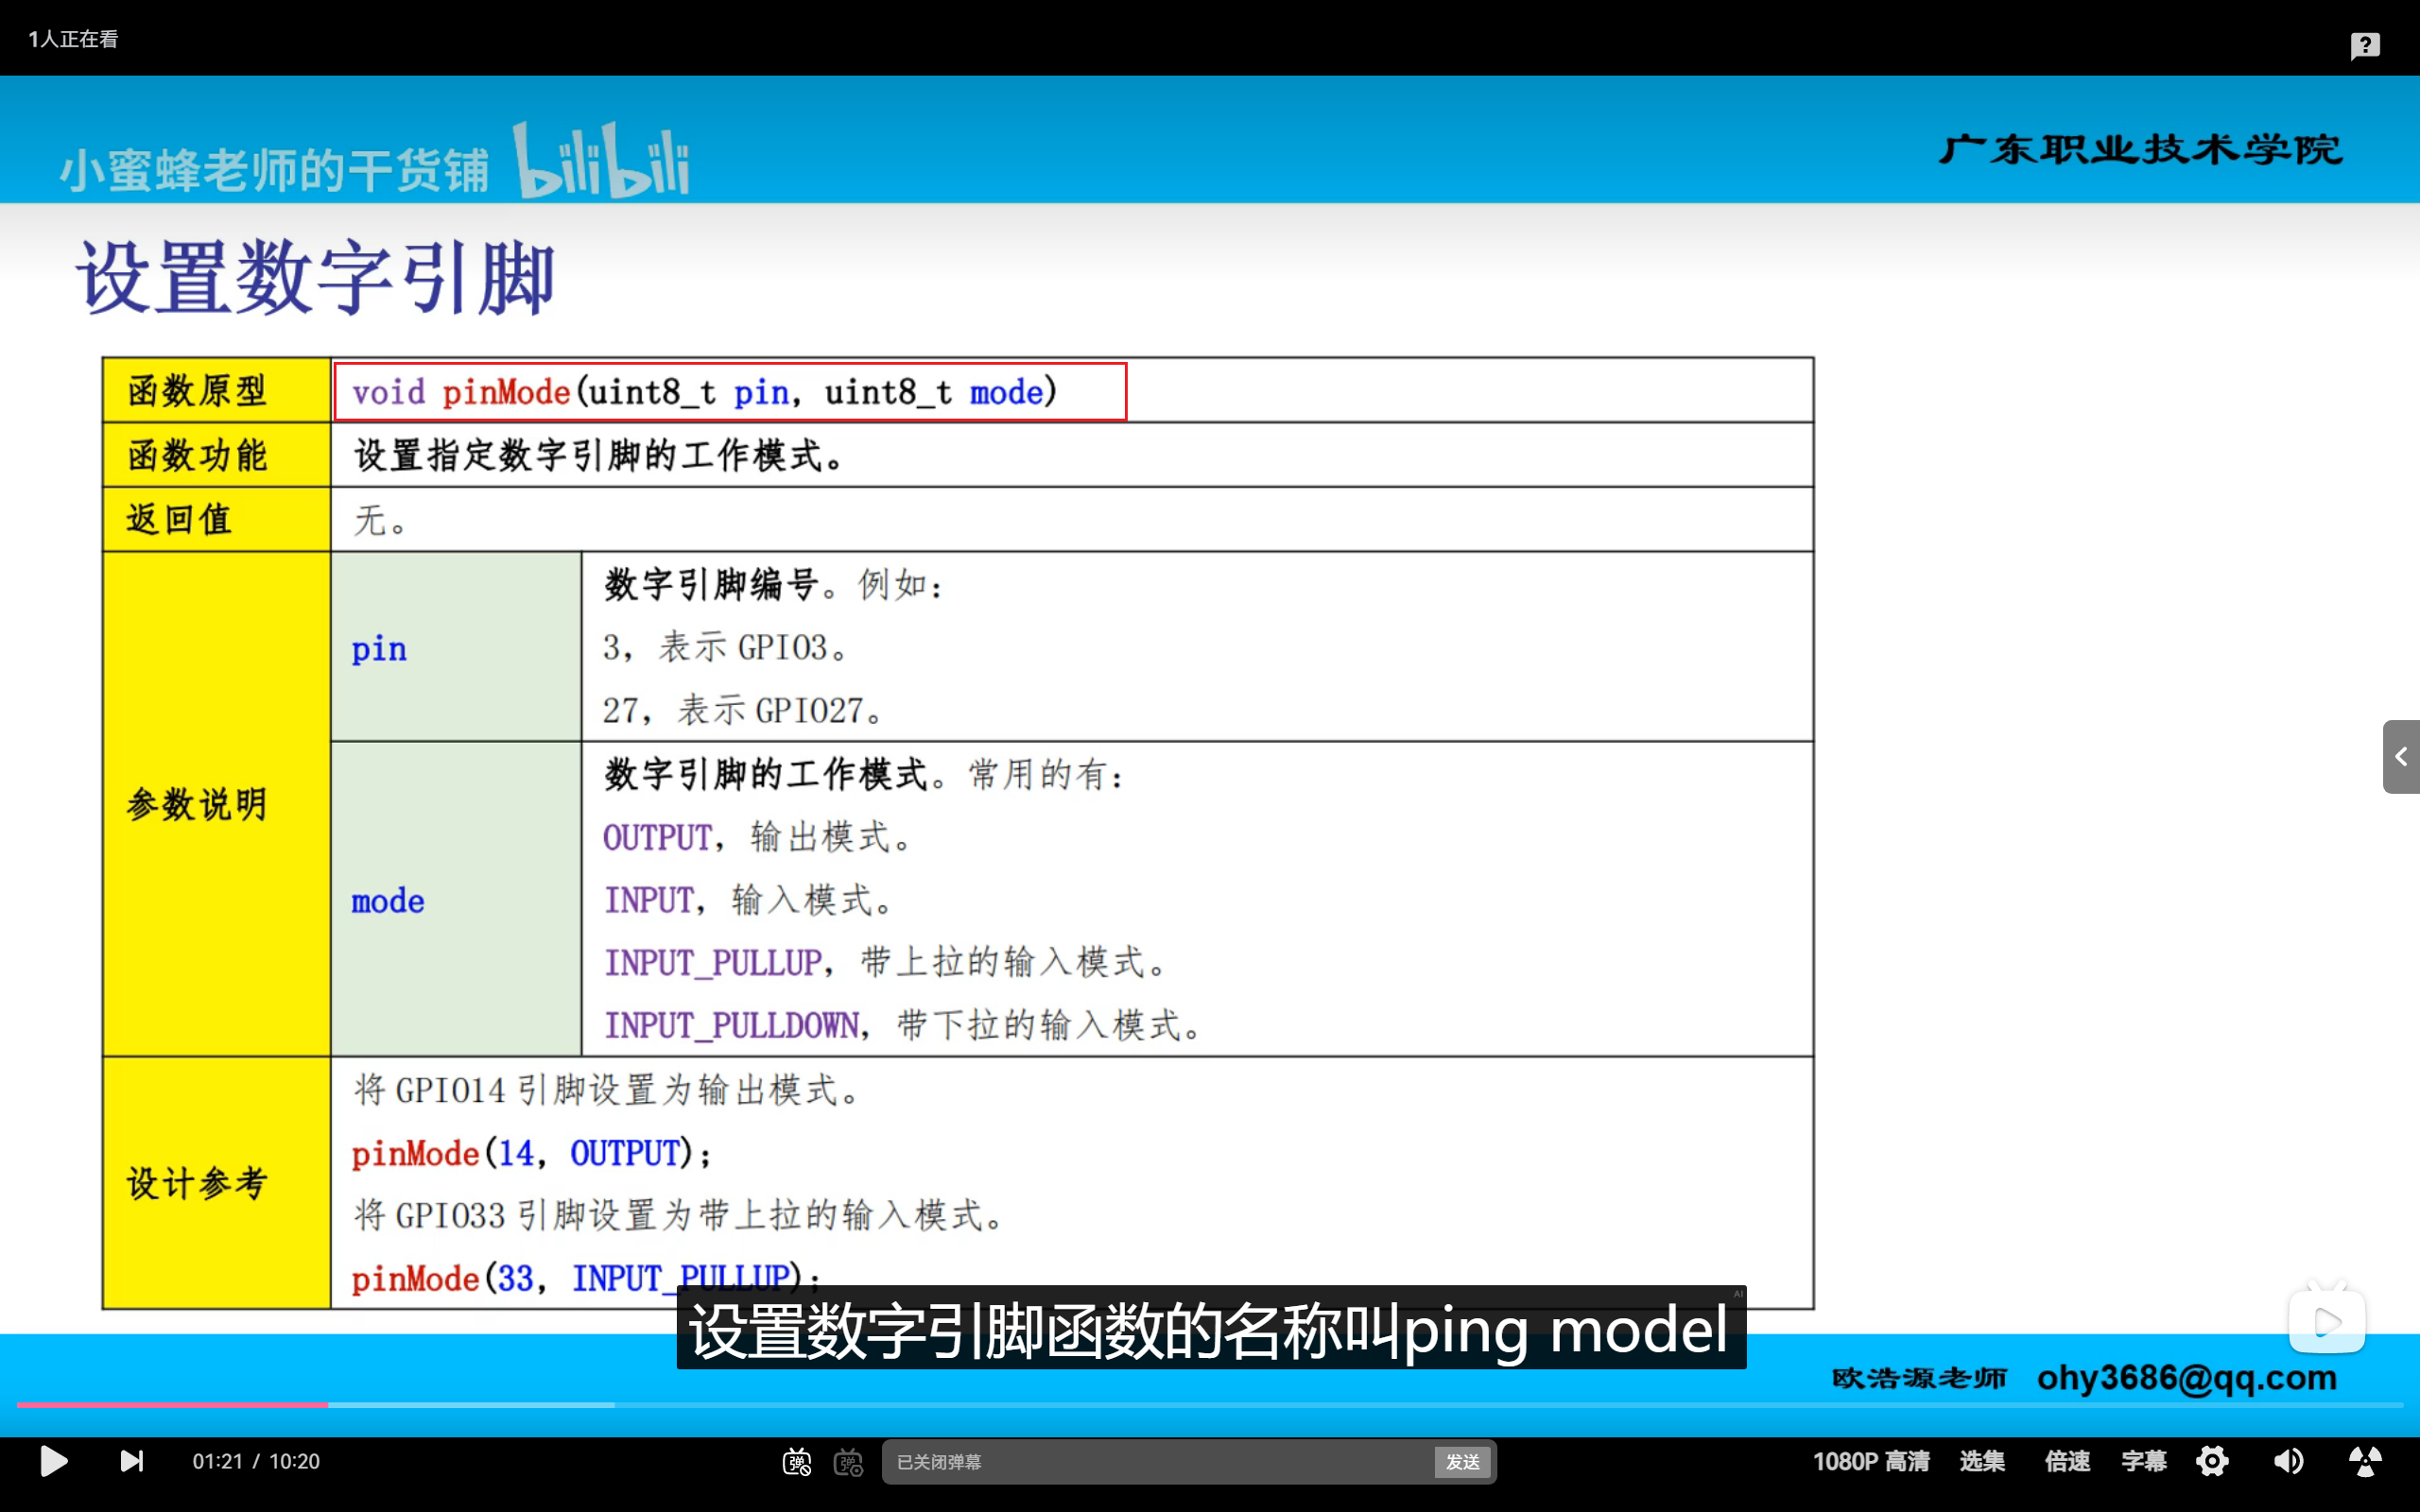
\includegraphics[width=\textwidth]{Figures/pinMode.png}
    \caption{pinMode}
    \label{fig:placeholder}
\end{figure}



函数名为: \textit{\textbf{void pinMode(参数一, 参数二)}}, 第一个参数为要初始化的引脚, 第二个参数为要设置的模式 
\newpage
\subsection{ GPIO引脚电平写入函数, 用于控制GPIO口的高低电平 }
\begin{figure}[h]
    \centering
    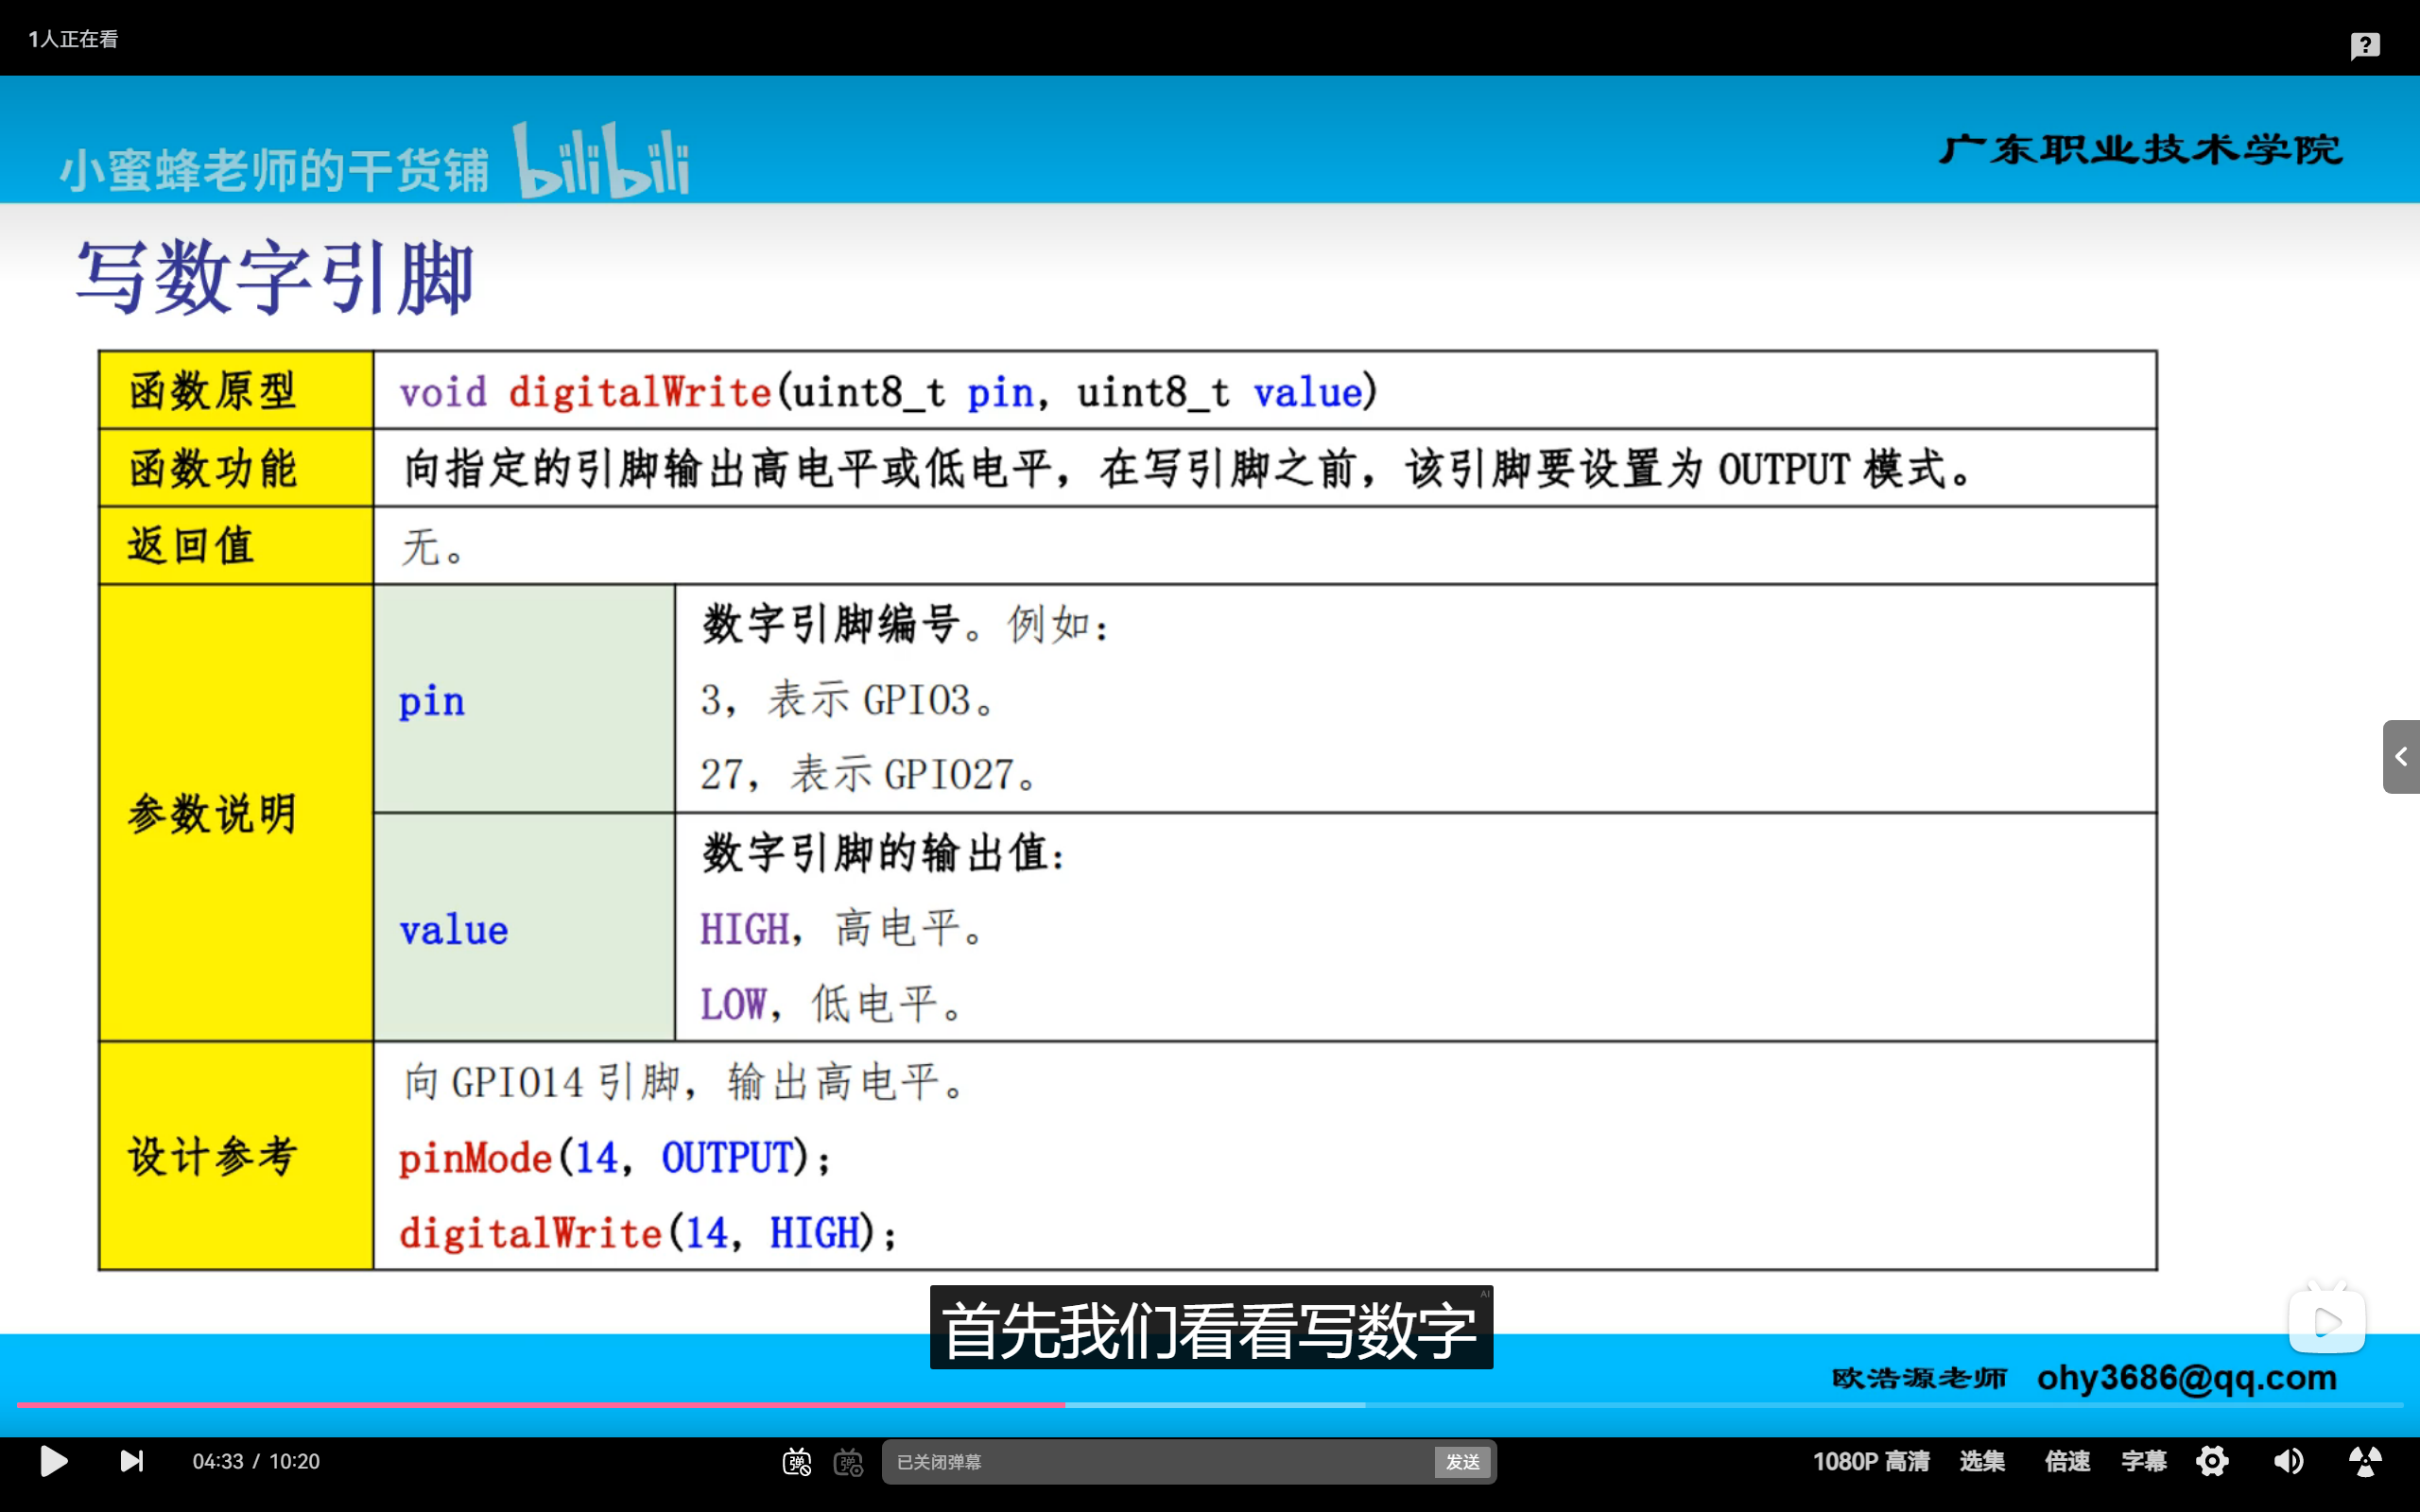
\includegraphics[width = \textwidth]{Figures/exemple.png}
    \caption{电平写入函数}
    
\end{figure}
函数名为: \textit{\textbf{digitalWrite(参数一,参数二)}}, 第一个参数表示引脚, 第二个参数表示Value(有HIGH和LOW)

\newpage
\subsection{ GPIO引脚电平读取函数, 用于获取GPIO口的高低电平 }
\begin{figure}[h]
    \centering
    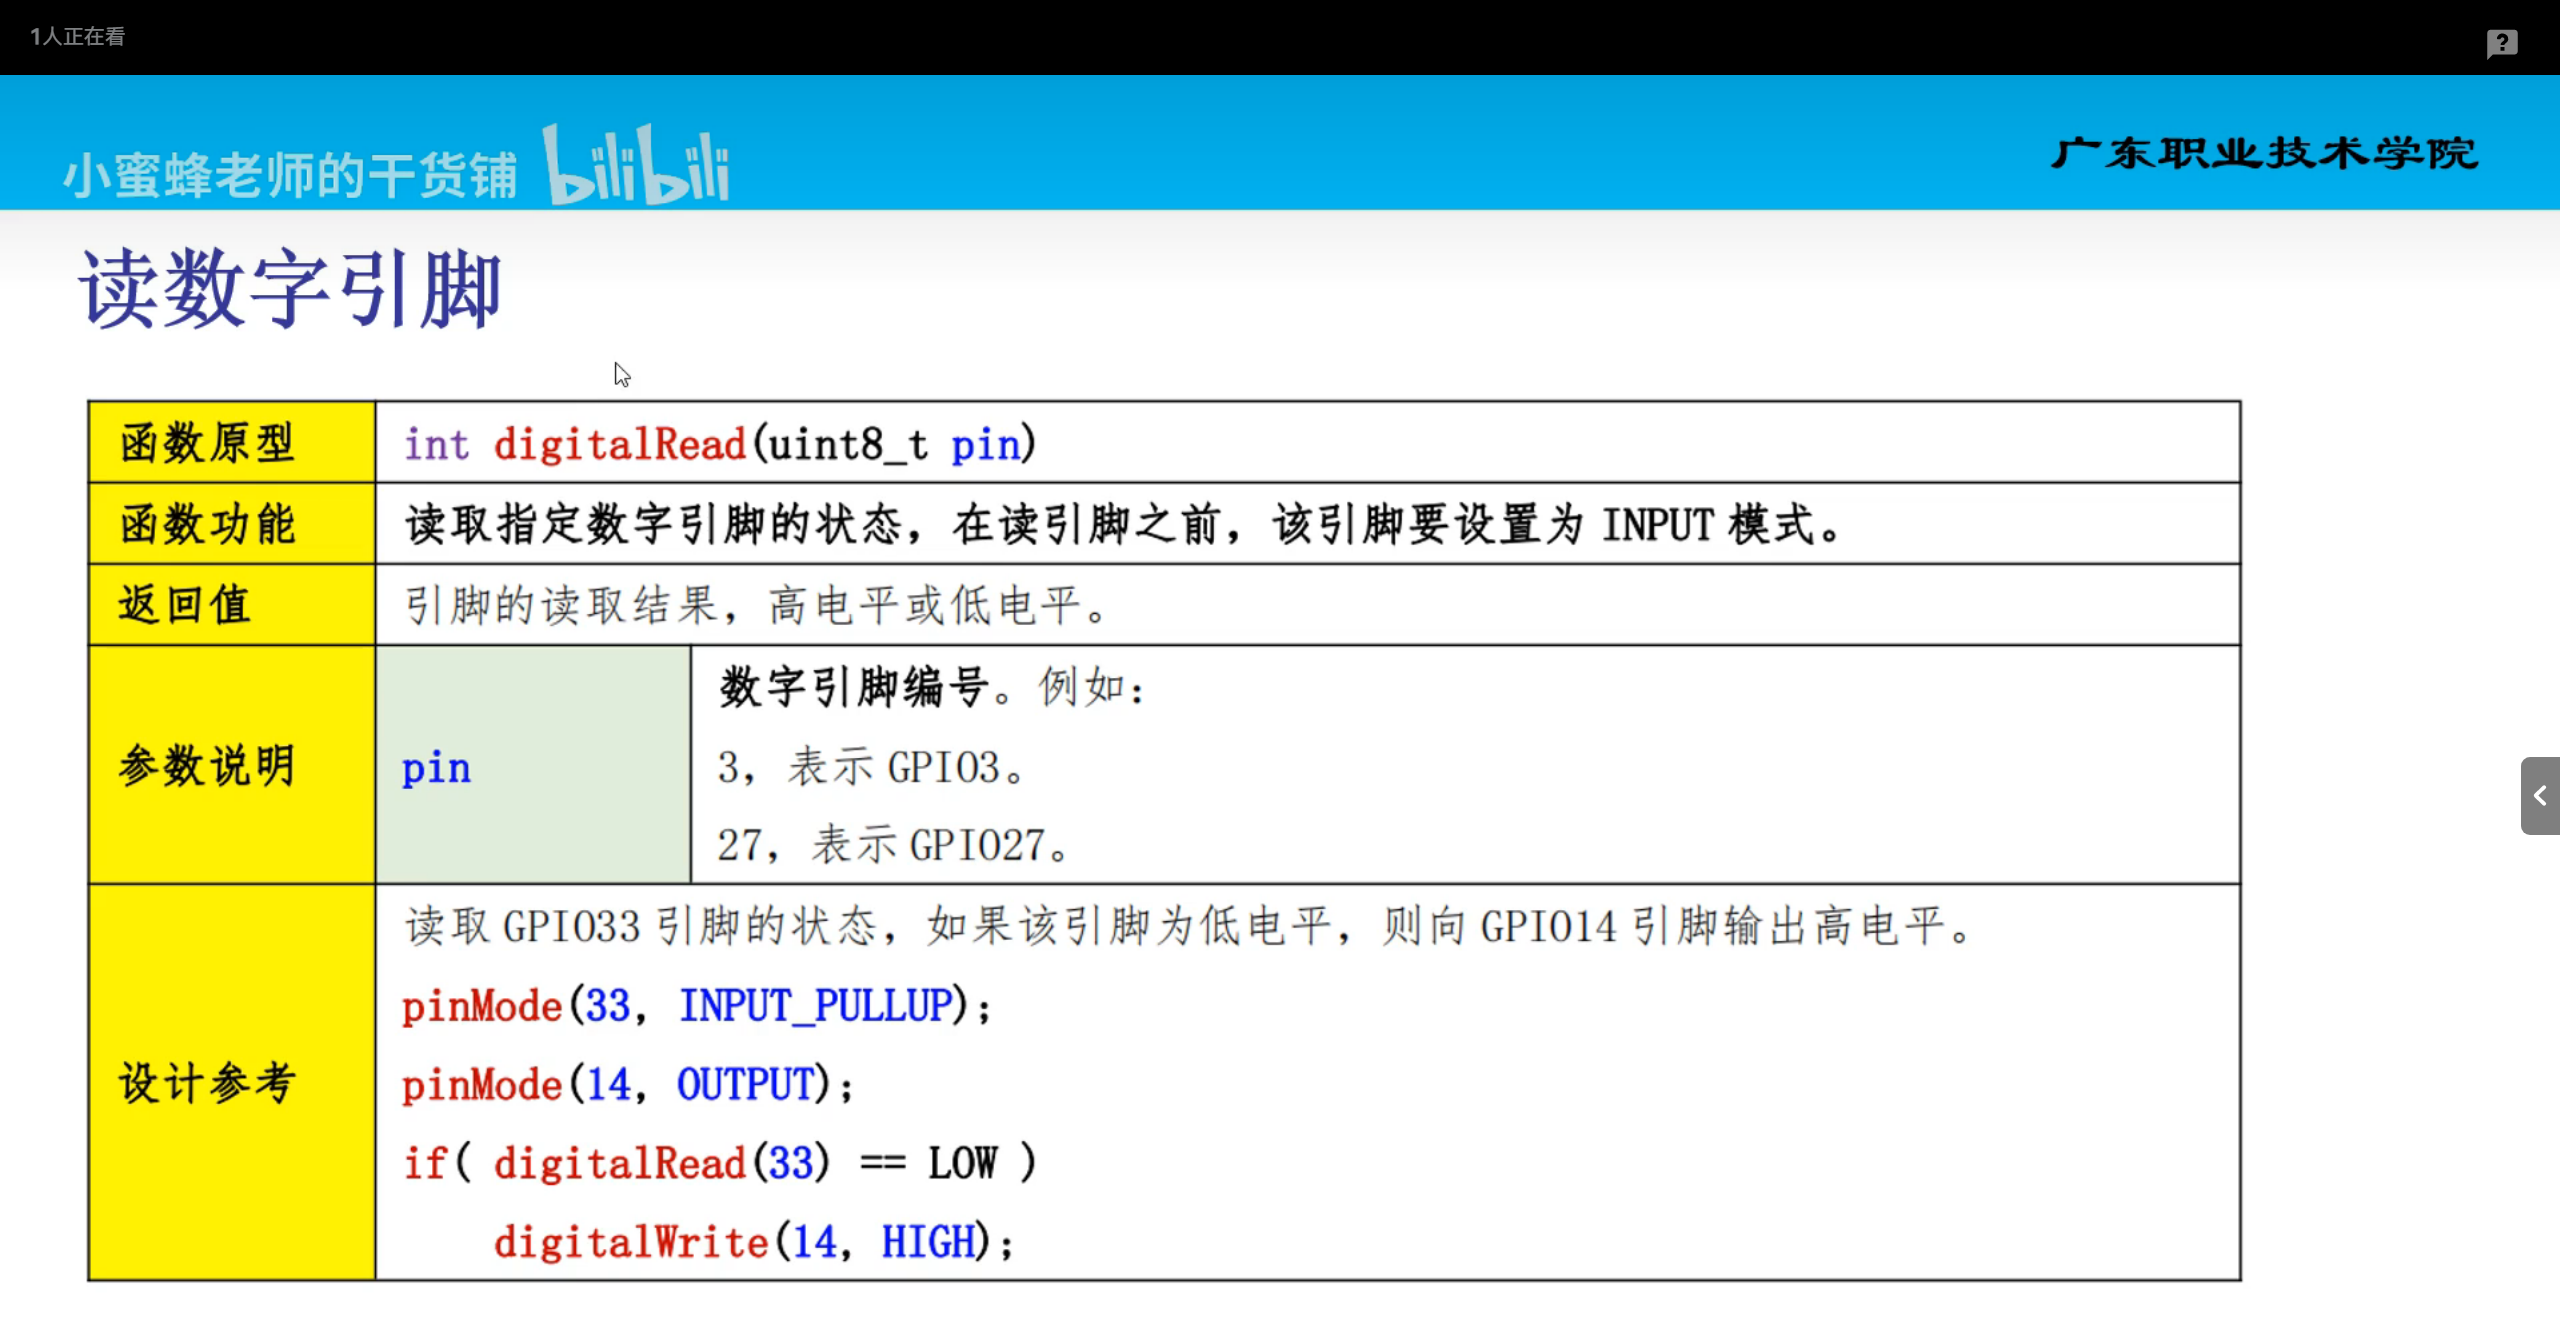
\includegraphics[width=\textwidth]{Figures/digitalRead.png}
    \caption{digitalRead}
   
\end{figure}
函数名为: \textit{\textbf{void digitalRead(参数一)}},参数一为要读取的引脚

